\documentclass[a4paper]{article}
\usepackage[utf8]{inputenc}
\usepackage{amsmath,amsfonts,amssymb,amsthm, mathrsfs}
%\usepackage{mathtools}
\usepackage{graphicx}
\usepackage{setspace}
\usepackage{comment}
\usepackage{multirow}
% \usepackage[a4paper, total={6in, 8in}]{geometry}
\usepackage[top=2.0cm, left=2.0cm, right=2.0cm, bottom=3.0cm]{geometry}
\usepackage[colorlinks = true, linkcolor = cyan, urlcolor  = cyan, citecolor = cyan, anchorcolor = cyan]{hyperref}
\usepackage{diagbox}


%\DeclareSymbolFont{letters}{OT1}{cmtt}{m}{n}
%\renewcommand{\familydefault}{\sfdefault}


\title{%
%\vspace{1em}
    \textsc{Exercises} \\
    \vspace{1mm}
    \large \textsc{Social Choice Theory}
}
\author{Wenjie Tu}
\date{Spring Semester 2022}

\setlength{\parindent}{0pt}
\setlength{\parskip}{1em}
%\onehalfspacing
\begin{document}

\maketitle

\section*{Part 1: Preliminaries}

\subsection*{Exercise 1.1}

\subsubsection*{(a)} 

\textit{Find an example of a binary relation that is quasi-transitive but not transitive.}

Let $X=\{x, y, z\}$. A binary relation $R$ on the set $X$ is as follows:
\[R=\{(x,y), (y,z), (z,y) \} \]

The asymmetric part is:
\[P=\{(x,y)\} \]

\begin{itemize}
    \item The induced asymmetric part $P=\{(x,y)\}$ is transitive, hence $R$ is quasi-transitive.
    \item $(x,y)\in R$ and $(y,z)\in R$ while $(x,z)\notin R$, a contradiction to transitivity.
\end{itemize}

Therefore $R=\{(x,y), (y,z), (z,y) \}$ is quasi-transitive but not transitive.

\subsubsection*{(b)}

\textit{Find an example of a binary relation that is acyclical but not quasi-transitive}

Let $X=\{x, y, z\}$. A binary relation $R$ on the set $X$ is as follows:
\[R=\{(x,y), (y,z) \} \]

Its asymmetric part $P$ is:
\[P=\{(x,y), (y,z) \} \]

\begin{itemize}
    \item Since $(x,z)\notin P$, $P$ is not transitive and $R$ is not quasi-transitive.
    \item Since $(z,x)\notin P$, $P$ has no cycle and $R$ is acyclical.
\end{itemize}


\subsubsection*{(c)}

\textit{Show that, if $R$ is transitive, then its induced $I$ is also transitive.}

Need to show:
\[xIy \land yIz \implies xIz \]

Proof:

We can rewrite induced $I$ into binary relation:

\[xIy\implies [xRy \land yRx] \]
\[yIz\implies [yRz \land zRy] \]

\[xRy \land yRz \implies xRz \quad \text{by transitivity} \]
\[yRx \land zRy \implies zRx \quad \text{by transitivity} \]

\[xRz \land zRx \implies xIz \]

\textbf{Extension}

\subsubsection*{(d)}

\textit{Find an example of binary relation that is irreflexive.}

Let $X$ be an arbitrary set. A binary relation $R$ on the set $X$ is given as $\varnothing$ and it is irreflexive.

\subsubsection*{(e)}

\textit{Find an example of binary relation that is both reflexive and irreflexive.}

Let $X=\varnothing$. Any binary relation on the set $X$ is $R=\varnothing$, hence it is both reflexible and irreflexive.

\subsubsection*{(f)}

\textit{Find an example of binary relation that is neither reflexive nor irreflexive.}

Let $X=\{x, y\}$, and a binary relation on $X$ is $R=\{(x, x)\}$.
\begin{itemize}
    \item $R$ is not reflexive because $(y,y)\notin R$ (a violation of reflexivity).
    \item $R$ is not irreflexive because $(x,x)\in R$ (a violation of irreflexivity).
\end{itemize}

\subsubsection*{(g)}

\textit{Find an example of binary relation that is both symmetric and asymmetric.}

Let $X$ be an arbitrary set and $R$ is an empty set on $X$ (i.e., $R=\varnothing$).

\begin{align*}
    \text{symmetric:} \qquad & xRy\implies yRx, \quad \forall x, y\in X \\
    \text{asymmetric:} \qquad & xRy\implies\neg yRx, \quad \forall x, y\in X
\end{align*}

According to the definitions of symmetry and asymmetry of the binary relation, we are not able to find any counter examples so such a binary relation $R$ is both symmetric and asymmetric.

Note:
\[\text{asymmetric} \implies \text{irreflexive} \]

\subsubsection*{(g)}

\textit{Find an example of binary relation that is anti-symmetric not but asymmetric.}

Let $X=\{x, y, z\}$ and a binary relation on $X$ is $R=\{(x,x), (y,y), (z,z) \}$
\begin{align*}
    \text{asymmetric:}\qquad & xRy \implies \neg yRx,\quad \forall x, y\in X \\
    \text{anti-symmetric:}\qquad & xRy \implies \neg yRx,\quad \forall x, y\in X \text{ with } x\neq y
\end{align*}

Note: anti-symmetric is weaker than asymmetric.

\subsection*{Exercise 1.2}

\subsubsection*{(a)}

$\succeq$ is a preference

\[x\sim y \]
\[y\succ z \]
\[z\succ w \]

\[G(\{w,x,y,z\})=\{x,y\} \]
\[M(\{w,x,y,z\})=\{x,y\} \]

\[R=\{(x,y), (y,x), (y,z), (z,w) \} \]

\subsubsection*{(b)}

\[M(\{x,y,z\}, R)=\{\}=G(\{x,y,z\}) \]

\subsection*{Exercise 1.3}

\subsubsection*{(a)}

We know that $x$ is chosen in the larger set (i.e. $C(\{x,y,z\})=\{x\}$), and we need to check whether $x$ is still chosen from all the possible subset containing $x$.

\[C(\{x,y\})=\{x\} \]
\[C(\{x,z\})=\{x\} \]

Hence, property $\alpha$ is satisfied.

We cannot find any two alternatives that are generate by the choice function. Hence, we cannot find a counter example that violates property $\beta$ (i.e. $\beta$ is satisfied).

\subsubsection*{(b)}

We know that $z$ is chosen from the larger set (i.e. $C(\{x,y,z\})=\{z\}$), and we need to check whether $z$ is still chosen from all the possible subset containing $z$.

Base relation:

\[C(\{x,z\})=\{x,z\} \]
\[C(\{y,z\})=\{z\} \]

Preference:
\[x\sim z \succ y \]

Hence, property $\alpha$ is satisfied.

We see that $\{x,z\}$ is chosen from the smaller set $\{x,z\}$ (i.e. $C(\{x,z\})=\{x,z\}$), and $z$ is chosen from the larger set $\{x,y,z\}$ while $x$ is not, hence a violation of property $\beta$.

\subsubsection*{(c)}

We know that $\{y,z\}$ is chosen from the larger set $\{x,y,z\}$, and we need to check whether $\{y,z\}$ is still chosen from all the possible subset containing $\{y,z\}$.

We see:
\[C(\{y,z\})=\{y,z\} \]

Hence, property $\alpha$ is satisfied.

We see that $\{y,z\}$ is chosen from the smaller set $\{y,z\}$, and $\{y,z\}$ is chosen from the larger set containing both $y$ and $z$. Hence, property $\beta$ is satisfied.


\subsection*{Exercise 1.4}

Shorthands for choices:
\begin{itemize}
    \item $P$: peatnuts
    \item $A$: apple juice
    \item $M$: mineral water
    \item $B$: beer
\end{itemize}

\subsubsection*{(a)}

\[X=\{P,A,M,B \} \]

\[C(\{P,A,M\})=\{P, A\} \]

\[C(\{P,A,M,B\})=\{P, B\} \]

$\beta$ is violated?

Better translation of the information:
\[X=\{PA, PM, PB \} \]

\[C(\{PA,PM\})=\{PA\} \]

\[C(\{PA,PM,PB\})=\{PB\} \]

$\beta$ is satisfied.

\section*{Part 2: The Problem of Social Choice}

\subsection*{Exercise 2.1}

\subsubsection*{(a)}

\begin{table}[!htbp]
    \centering
    \begin{tabular}{c|c|}
        \# & preferences         \\ 
        \hline
        1  & $x\: P\: y\: P\: z$ \\
        1  & $y\: P\: z\: P\: x$ \\
        1  & $z\: P\: x\: P\: y$ \\
        \hline
    \end{tabular}
\end{table}

\begin{table}[!htbp]
    \centering
    \begin{tabular}{ccc}
        \hline
        Pairwise comparison & Votes               & Social preference  \\ 
        \hline
        $x\: \text{vs.} y$  & $2\: \text{vs.} 1$  & $xPy$              \\
        $x\: \text{vs.} z$  & $1\: \text{vs.} 2$  & $zPx$              \\
        $y\: \text{vs.} z$  & $2\: \text{vs.} 1$  & $yPz$              \\
        \hline
    \end{tabular}
\end{table}

This leads to an outcome that is not transitive and not acyclical.

There is no Condorcet winner (loser) as each alternative loses in the pairwise voting at once.

\subsubsection*{(b)}

Fix any $R^*\in R$, let $\mathscr{A}=\{(R^*, R^*,\cdots, R^*) \}$. In other words, all individuals share the same preference. In this example, the pairwise majority voting is an SWF.

\subsection*{Exercise 2.2}

When $m=2$, PV, IR, PM, CO, and BC are identical. They all collapse to the majority voting method.

\subsection*{Exercise 2.3}

\begin{table}[!htbp]
    \centering
    \begin{tabular}{c|c|}
        \# & preferences         \\ 
        \hline
        2  & $x\: P\: w\: P\: y\: P\: z$ \\
        2  & $y\: P\: w\: P\: z\: P\: x$ \\
        1  & $w\: P\: z\: P\: x\: P\: y$ \\
        \hline
    \end{tabular}
\end{table}

\subsubsection*{PV:}

In plurality voting, we only consider the top-ranked alternatives given by voters.
\[x\: I\: y\: P\: w\: P\: z  \]

\subsubsection*{IR:}

\begin{itemize}
    \item Stage 1: $z$ is eliminated
    \item Stage 2: $w$ is eliminated
    \item Stage 3: $x$ wins with 3 votes (majority)
\end{itemize}

\subsubsection*{PM:}


\begin{table}[!htbp]
    \centering
    \begin{tabular}{ccc}
        pairwise comparison & votes  & binary relation \\
        \hline 
        $w:x$  & $3:2$  & $wPx$           \\
        $w:y$  & $3:2$  & $wPy$           \\
        $w:z$  & $5:0$  & $wPz$           \\
        $x:y$  & $3:2$  & $xPy$           \\
        $x:z$  & $2:3$  & $zPx$           \\
        $y:z$  & $4:1$  & $yPz$           \\
        \hline
    \end{tabular}
\end{table}

The pairwise majority voting method delivers a Condorcet winner $w$ but there exists a cycle in $x, y, z$.

\subsubsection*{CO:}

\begin{table}[!htbp]
    \centering
    \begin{tabular}{c|c|c|c|c|c}
            & $w$  & $x$  & $y$  & $z$  & $\sum$ \\
        \hline 
        $w$ &      & $+1$ & $+1$ & $+1$ & $3$    \\
        \hline 
        $x$ & $-1$ &      & $+1$ & $-1$ & $-1$   \\
        \hline
        $y$ & $-1$ & $-1$ &      & $+1$ & $-1$   \\
        \hline
        $x$ & $-1$ & $+1$ & $-1$ &      & $-1$   \\
        \hline
    \end{tabular}
\end{table}

Copeland method delivers the social preference $w \: P \: x \: I \: y \: I \: z$.

\subsubsection*{BC:}

\begin{table}[!htbp]
    \centering
    \begin{tabular}{c|c|cccc|}
        \# & preferences                  & $w$  & $x$  & $y$  & $z$ \\ 
        \hline
        2  & $x\: P\: w\: P\: y\: P\: z$  & $2$  & $3$  & $1$  & $0$ \\
        2  & $y\: P\: w\: P\: z\: P\: x$  & $2$  & $0$  & $3$  & $1$ \\
        1  & $w\: P\: z\: P\: x\: P\: y$  & $3$  & $1$  & $0$  & $2$ \\
        \hline
           &                              & $11$ & $7$  & $8$  & $4$ \\
        \hline
    \end{tabular}
\end{table}

Borda Count method delivers the social preference $wPyPxPz$

\subsubsection*{EM:}

There exists at least one individual who ranks $x, y, w$ as his/her top preference, hence the Pareto efficient set is $X^E=\{w, x, y\}$. All individuals strictly prefer $w$ over $z$, hence $z$ is strictly dominated by $w$. $X^I=\{z\}$.

Pareto Efficient Method delivers the social preference $wIxIyPz$.

\subsubsection*{PE:}

\begin{table}[!htbp]
    \centering
    \begin{tabular}{cc}
        pairwise comparison & Pareto extension rule \\
        \hline 
        $w:x$  & $wIx$           \\
        $w:y$  & $wIy$           \\
        $w:z$  & $wPz$           \\
        $x:y$  & $xIy$           \\
        $x:z$  & $zIx$           \\
        $y:z$  & $yIz$           \\
        \hline
    \end{tabular}
\end{table}

Pareto Extension Rule delivers an outcome that violates transitivity but is quasi-transitive. This is SDF but not SWF.

\subsection*{Exercise 2.4}

\subsubsection*{(a)}

\begin{table}[!htbp]
    \centering
    \begin{tabular}{c|c|}
        \# & preferences         \\ 
        \hline
        2  & $x\: P\: z\: P\: y$ \\
        2  & $y\: P\: z\: P\: x$ \\
        1  & $z\: P\: y\: P\: x$ \\
        \hline
    \end{tabular}
\end{table}

Applying IR:
\begin{itemize}
    \item Stage 1: $z$ is eliminated.
    \item Stage 2: $y$ wins with 3 votes (majority).
\end{itemize}

\begin{table}[!htbp]
    \centering
    \begin{tabular}{ccc}
        pairwise comparison & votes  & binary relation \\
        \hline 
        $x:y$  & $2:3$  & $yPx$           \\
        $x:z$  & $2:3$  & $zPx$           \\
        $y:z$  & $2:3$  & $zPy$           \\
        \hline
    \end{tabular}
\end{table}

\begin{itemize}
    \item $z$ wins all pairwise comparison hence a Condorcet winner.
    \item IR is not a Condorcet method.
\end{itemize}

\subsubsection*{(b)}

Proof by contradiction:

No, a Condorcet winner is Pareto efficient, otherwise it would lose at least one pairwise vote.

\subsubsection*{(c)}

We can construct the following example resulting $x$ to be a Condorcet winner:

\begin{table}[!htbp]
    \centering
    \begin{tabular}{c|c|}
        \# & preferences         \\ 
        \hline
        2  & $x\: P\: y$ \\
        1  & $y\: P\: x$ \\
        \hline
    \end{tabular}
\end{table}

There is no Pareto dominance between $x$ and $y$ so EM delivers social indifference between $x$ and $y$ (i.e. $xIy$).

Same argument for PE.

\subsection*{Exercise 2.5}

\subsubsection*{(a)}

For arbitrary values of $m$:
\begin{itemize}
    \item Anti-plurality voting and rejection voting are equivalent.
    \item Nameless example I and nameless example II are equivalent.
\end{itemize}

For $m=3$:
\begin{itemize}
    \item Anti-plurality voting and rejection voting are equivalent.
    \item Borda count, nameless example I, and nameless example II are equivalent.
\end{itemize}

\subsubsection*{(b)}

\[s=(m, m-1, \cdots, 1) \]

\subsubsection*{(c)}

\[s=(m^2, (m-1)^2, \cdots, 1^2) \]

\subsection*{Exercise 2.6}

\begin{table}[!htbp]
    \centering
    \begin{tabular}{c|c|cccc|}
        \# & preferences                  & $v$  & $x$  & $y$  & $z$ \\ 
        \hline
        1  & $x\: P\: z\: P\: v\: P\: y$  & $1$  & $3$  & $0$  & $2$ \\
        1  & $y\: P\: z\: P\: v\: P\: x$  & $1$  & $0$  & $3$  & $2$ \\
        1  & $v\: P\: z\: P\: y\: P\: x$  & $3$  & $0$  & $1$  & $2$ \\
        1  & $x\: P\: y\: P\: v\: P\: z$  & $1$  & $3$  & $2$  & $0$ \\
        \hline
           &                              & $6$ & $6$  & $6$  & $6$ \\
        \hline
    \end{tabular}
\end{table}

$s^1$ delivers social preference $vIxIyIz$

\begin{table}[!htbp]
    \centering
    \begin{tabular}{c|c|cccc|}
        \# & preferences                  & $v$  & $x$  & $y$  & $z$ \\ 
        \hline
        1  & $x\: P\: z\: P\: v\: P\: y$  & $1/4$  & $1$  & $0$  & $3/4$ \\
        1  & $y\: P\: z\: P\: v\: P\: x$  & $1/4$  & $0$  & $1$  & $3/4$ \\
        1  & $v\: P\: z\: P\: y\: P\: x$  & $1$  & $0$  & $1/4$  & $3/4$ \\
        1  & $x\: P\: y\: P\: v\: P\: z$  & $1/4$  & $1$  & $3/4$  & $0$ \\
        \hline
           &                              & $7/4$ & $8/4$  & $8/4$  & $9/4$ \\
        \hline
    \end{tabular}
\end{table}

$s^2$ delivers social preference $zPxIyPv$

\begin{table}[!htbp]
    \centering
    \begin{tabular}{c|c|cccc|}
        \# & preferences                  & $v$  & $x$  & $y$  & $z$ \\ 
        \hline
        1  & $x\: P\: z\: P\: v\: P\: y$  & $1/4$  & $1$  & $0$  & $1/2$ \\
        1  & $y\: P\: z\: P\: v\: P\: x$  & $1/4$  & $0$  & $1$  & $1/2$ \\
        1  & $v\: P\: z\: P\: y\: P\: x$  & $1$  & $0$  & $1/4$  & $1/2$ \\
        1  & $x\: P\: y\: P\: v\: P\: z$  & $1/4$  & $1$  & $1/2$  & $0$ \\
        \hline
           &                              & $7/4$ & $8/4$  & $7/4$  & $6/4$ \\
        \hline
    \end{tabular}
\end{table}

$s^3$ delivers social preference $xPvIyPz$

\section*{Part 3: Arrow's Theorem}

\subsection*{Exercise 3.1}

\subsubsection*{(a) Plurality voting (PV)}

\underline{[I] Independence of Irrelevant Alternatives Axiom is violated. }

The counter example is given as follows:

\begin{table}[!htbp]
    \centering
    \begin{tabular}{c|c|}
        $\mathbf{R}$ & preferences         \\ 
        \hline
        2  & $x\: P\: y\: P\: z$ \\
        1  & $y\: P\: x\: P\: z$ \\
        1  & $x\: P\: z\: P\: y$ \\
        \hline 
        $f^{PV}$ & $x\: P\: y\: P\: z$
    \end{tabular}
    \qquad $\to$ \qquad
    \centering
    \begin{tabular}{c|c|}
        $\mathbf{R'}$ & preferences         \\ 
        \hline
        2  & $z\: P\: x\: P\: y$ \\
        1  & $y\: P\: x\: P\: z$ \\
        1  & $x\: P\: z\: P\: y$ \\
        \hline 
        $f^{PV}$ & $z\: P\: y\: I\: x$
    \end{tabular}
\end{table}

Note: $z$ is the irrelevant alternative. We change the preferences for $z$ for the first two people while maintaining the relative positions for $x$ and $y$ (i.e. $xPy$). From $\mathbf{R}\to\mathbf{R'}$, we see social preference between $x$ and $y$ changes, hence a violation of [I].

\underline{[P] Weak Pareto Principle is violated. }

The counter example is given as follows:

\begin{table}[!htbp]
    \centering
    \begin{tabular}{c|c|}
        $\mathbf{R}$ & preferences         \\ 
        \hline
        2  & $z\: P\: x\: P\: y$ \\
        \hline 
        $f^{PV}$ & $z\: P\: x\: I\: y$
    \end{tabular}
\end{table}

\underline{[U] Universality is satisfied. }

\begin{itemize}
    \item Plurality voting (PV) is well-defined method and always applicable as there are no constraints in definition/preferences.
    \item The resulting outcomes are preferences as plurality voting method is a ranking method based on numbers/votes. Numbers are transitive, hence outcomes are transitive (PV is a SWF).
\end{itemize}

\underline{[D] Non-dictatorship is satisfied.} 

Each individual has only one vote. In order to impose the own preference on the whole society, the dictator must have ``majority'' votes, which is not possible for plurality voting where each individual has one single vote.

Or proof by contradiction.

\subsubsection*{(b) Pairwise majority voting (PM)}

\underline{[I] Independence of Irrelevant Alternatives Axiom is satisfied. }

Pairwise majority voting method is a pairwise method by construction. To determine the ranking between $x$ and $y$, we do pairwise comparison. If preferences between $x$ and $y$ do not change, the outcome does not change.

\underline{[D] Non-dictatorship is satisfied.} 

As long as the majority is against you, you cannot enforce your own preference on the society. This holds for everybody. Nobody can be a dictator.

\underline{[P] Weak Pareto Principle is satisfied.}

If everybody has a strict preference for $x$ over $y$, the outcome will be an unanimous vote for $x$ over $y$ as we only do pairwise comparison, hence a strict preference for $x$ over $y$ for the society.

\underline{[U] Universality is violated.}

A counter example is constructed as follows:

\begin{table}[!htbp]
    \centering
    \begin{tabular}{c|c|}
        \# & preferences         \\ 
        \hline
        1  & $x\: P\: y\: P\: z$ \\
        1  & $y\: P\: z\: P\: x$ \\
        1  & $z\: P\: x\: P\: y$ \\
        \hline
    \end{tabular}
\end{table}

The example given above leads to an acyclical preferences. This is not a SWF on the full domain. We can easily get violations of acyclicity and transitivity.

\subsubsection*{(c) Copeland method (CO)}

\underline{[U] Universality is satisfied.}

Copeland method by definition is a number-based voting method and hence it is always applicable as numbers are always transitive.

\underline{[D] Non-dictatorship is satisfied.} 

As long as the majority is against you, you cannot enforce your own preference on the society. This holds for everybody. Nobody can be a dictator.

\underline{[P] Weak Pareto Principle is satisfied.}

Suppose $x$ strictly Pareto dominates $y$, under Copeland method $y$ loses every pairwise vote that $x$ loses. In other words, whenever $x$ loses, $y$ loses as well. 
\[CO(x, \mathbf{R}) \geq CO(y,\mathbf{R})+2 \]

\underline{[I] Independence of Irrelevant Alternatives Axiom is violated.}

A counter example is constructed as follows:

\begin{table}[!htbp]
    \centering
    \begin{tabular}{c|c|}
        $\mathbf{R}$ & preferences         \\ 
        \hline
        1  & $x\: P\: y\: P\: z$ \\
        1  & $y\: P\: x\: P\: z$ \\
        \hline 
        $f^{CO}$ & $x\: I\: y\: P\: z$
    \end{tabular}
    \qquad $\to$ \qquad
    \centering
    \begin{tabular}{c|c|}
        $\mathbf{R'}$ & preferences         \\ 
        \hline
        1  & $x\: P\: y\: P\: z$ \\
        1  & $y\: P\: z\: P\: x$ \\
        \hline 
        $f^{CO}$ & $y\: P\: x\: P\: z$
    \end{tabular}
\end{table}

Note: $z$ is the irrelevant alternative. We change the preference for $z$ for the second person while maintaining the relative positions for $x$ and $y$ (i.e. $xPy$). From $\mathbf{R}\to\mathbf{R'}$, we see social preference between $x$ and $y$ changes, hence a violation of [I].

\subsubsection*{(d) Borda count (BC)}

\underline{[D] Non-dictatorship is satisfied.} 

Borda count method is formulated in a linear way for scoring vector and all votes use the same scoring vector, hence no dictatorship possible.

\underline{[U] Universality is satisfied.}

Borda count is a number-based voting method so it always leads to transitive preferences. It is applicable to all preference profiles as there are no constraints in definition.

\underline{[P] Weak Pareto Principle is satisfied.}

By definition, if $xP_i y\:\forall i$, 
\[BC(x, \mathbf{R})\geq BC(x, \mathbf{R}) + n \]
Hence, the society strictly prefers $x$ over $y$.

\underline{[I] Independence of Irrelevant Alternatives Axiom is violated.}

A counter example is constructed as follows:

\begin{table}[!htbp]
    \centering
    \begin{tabular}{c|c|}
        $\mathbf{R}$ & preferences         \\ 
        \hline
        1  & $x\: P\: y\: P\: z$ \\
        1  & $y\: P\: x\: P\: z$ \\
        \hline 
        $f^{BC}$ & $x\: I\: y\: P\: z$
    \end{tabular}
    \qquad $\to$ \qquad
    \centering
    \begin{tabular}{c|c|}
        $\mathbf{R'}$ & preferences         \\ 
        \hline
        1  & $x\: P\: y\: P\: z$ \\
        1  & $y\: P\: z\: P\: x$ \\
        \hline 
        $f^{BC}$ & $y\: P\: x\: P\: z$
    \end{tabular}
\end{table}

Note: $z$ is the irrelevant alternative. We change the preference for $z$ for the second person while maintaining the relative positions for $x$ and $y$ (i.e. $xPy$). From $\mathbf{R}\to\mathbf{R'}$, we see social preference between $x$ and $y$ changes, hence a violation of [I].

\subsubsection*{(e) Pareto Efficiency Method (EM)}

\underline{[D] Non-dictatorship is satisfied.} 

Proof by contradiction: suppose there exists a dictator who strictly prefers $x$ over $y$, the society is supposed to strictly prefer $x$ over $y$. Now there is an individual who strictly prefers $y$ over $x$, by definition of Pareto Efficiency Method, the society should be indifferent between $x$ and $y$ as there is no Pareto dominance between $x$ and $y$.

\underline{[P] Weak Pareto Principle is violated.}

\begin{table}[!htbp]
    \centering
    \begin{tabular}{c|c|}
        \# & preferences         \\ 
        \hline
        2  & $z\: P\: x\: P\: y$ \\
        \hline
        $f^{EM}$ & $z\: P\: x\: I\: y$
    \end{tabular}
\end{table}

\begin{itemize}
    \item $X^E=\{z \}$
    \item $X^I=\{x,y \}$
\end{itemize}

All individuals strictly prefer $x$ over $y$ but by applying Pareto Efficiency Method the society is indifferent between $x$ and $y$, hence a violation of Weak Pareto Principle.

\underline{[I] Independence of Irrelevant Alternatives Axiom is violated.}

A counter example is constructed as follows:

\begin{table}[!htbp]
    \centering
    \begin{tabular}{c|c|}
        $\mathbf{R}$ & preferences         \\ 
        \hline
        2  & $z\: P\: x\: P\: y$ \\
        \hline 
        $f^{EM}$ & $z\: P\: x\: I\: y$
    \end{tabular}
    \qquad $\to$ \qquad
    \centering
    \begin{tabular}{c|c|}
        $\mathbf{R'}$ & preferences         \\ 
        \hline
        2  & $x\: P\: y\: P\: z$ \\
        \hline 
        $f^{EM}$ & $x\: P\: y\: I\: z$
    \end{tabular}
\end{table}

Note: $z$ is the irrelevant alternative. We change the preferences for $z$ while maintaining the relative positions for $x$ and $y$ (i.e. $xPy$) for all individuals. From $\mathbf{R}\to\mathbf{R'}$, we see social preference between $x$ and $y$ changes, hence a violation of [I].

\underline{[U] Universality is satisfied.}

\begin{itemize}
    \item It is well-defined and always applicable.
    \item It always gives us preferences with at most two indifference classes.
\end{itemize}

\subsubsection*{(f) The preference of society coincides with the preference of individual $h\in N$}

\underline{[D] Non-dictatorship is violated.} 

By definition, the individual $h$ can always impose the own preference on the whole society and hence a dictator.

\underline{[U] Universality is satisfied.}

\begin{itemize}
    \item There are obviously no constraints built into the method and it is always applicable no matter how people's preferences look like.
    \item The dictator's preference is a preference. By definition of this method, the social preference will be a preference.
\end{itemize}

\underline{[P] Weak Pareto Principle is satisfied.}

If everybody strictly prefers $x$ over $y$, then the dictator also strictly prefers $x$ over $y$ because the dictator is one of those people.

\underline{[I] Independence of Irrelevant Alternatives Axiom is satisfied.}

Social preference is only determined by the dictator's preference. [I] holds for a single individual hence it also holds for the society with dictatorship. 

\subsubsection*{(g) Construct an example where all axioms but [P] are satisfied}

Fix any $R^*\in R$ and define $f(\mathbf{R})=R^*\:\forall\:\mathbf{R}\in\mathscr{R}^{U}$
\begin{itemize}
    \item [P] is violated
    \item [I] is satisfied
    \item [U] is satisfied. The outcome will be a preference and the method is well-defined on the universal domain
    \item [D] is satisfied. $R^*$ is arbitrary. Only the rule maker decides the dictator. Voters themselves do not know which one of them will be the dictator.
\end{itemize}

\subsection*{Exercise 3.2}

[$\mathrm{\bar{M}}$] is violated.

A counter example is constructed as follows:

\begin{table}[!htbp]
    \centering
    \begin{tabular}{c|c|}
        $\mathbf{R}$ & preferences         \\ 
        \hline
        2  & $x\: P\: z\: P\: y$ \\
        2  & $y\: P\: z\: P\: x$ \\
        1  & $z\: P\: x\: P\: y$ \\
        \hline 
           & $x$ wins
    \end{tabular}
    \qquad $\to$ \qquad
    \centering
    \begin{tabular}{c|c|}
        $\mathbf{R'}$ & preferences         \\ 
        \hline
        2  & $x\: P\: z\: P\: y$ \\
        2  & $z\: P\: y\: P\: x$ \\
        1  & $z\: P\: x\: P\: y$ \\
        \hline 
           & $z$ wins
    \end{tabular}
\end{table}

[$\mathrm{\bar{D}}$] is satisfied.

Proof by contradiction.

[$\mathrm{\bar{U}}$] is satisfied.

\begin{itemize}
    \item People are allowed to express whatever preferences they have. We have well-specified tie-breaking rules such that at the end there will always be a winner even if we go to the last stage.
    \item It is a well-specified method on the universal domain.
\end{itemize}

[$\mathrm{\bar{P}}$] is satisfied.

Suppose $yP_i x\:\forall i$
\begin{enumerate}
    \item As long as $y$ is around, $x$ gets zero votes
    \item $y$ can be eliminated only if it gets zero votes
    \item Updated votes do not change after elimination of alternatives with zero votes
    \item Either now or after some steps $x$ will be eliminated
    \item $x$ cannot be the winner
\end{enumerate}

\subsection*{Exercise 3.3}

\subsubsection*{(a)}

\begin{itemize}
    \item Consider the case where there is a Pareto ranking between those two alternatives. Everybody weakly prefers $x$ over $y$ and at least one person strictly prefers $x$ over $y$, then we do have a Pareto comparison between those two. In this case, both Pareto efficiency method (EM) and the Pareto extension rule (PE) will deliver the same outcome, which is strict social preference for $x$ over $y$.
    \item If there is no Pareto ranking between those two alternatives, by Pareto efficiency method (EM), both alternatives are Pareto efficient, which leads to a social indifference between those two alternatives. Pareto extension rule (PE) proceeds in a pairwise fashion, namely comparing alternatives pairwise. If there is no Pareto ranking between those two, we also get social indifference.
\end{itemize}
We therefore conclude that both methods are the same if $m=2$.

Both methods under $m=2$ are SWFs. Transitivity is usually the problem when there are more than two alternatives. However, transitivity is no longer a problem with two alternatives. Hence, transitivity is trivially satisfied in this case. It is complete because you can compare these two alternatives one way or the other. PE is always a SWF no matter how many alternatives you have. 

\subsubsection*{(b)}

In previous question, we have argued that both EM and PE are the same when $m=2$ so in this question we will not explicitly state which method.

\underline{[PR] is violated.}

A counter example is constructed as follows:
\begin{align*}
    f(+1, +1, -1, -1)&=0 \\
     & \downarrow        \\
    f(+1, +1, +1, -1)&=0 
\end{align*}

\underline{[N] is satisfied.}

There is no bias in favor of any alternatives. In particular, if everybody's preference switches to exactly the opposite, the social preference should also switch to exactly the opposite.

Case 1: $x$ Pareto dominates $y$
\begin{align*}
    f(+1, 0, +1, 0, 0) &= +1 \\
                       & \downarrow \\
    f(-1, 0, -1, 0, 0) &= -1                   
\end{align*}

Case 2: no Pareto dominance
\begin{align*}
    f(+1, +1, -1, -1) &= 0 \\
                      & \downarrow \\
    f(-1, -1, +1, +1) &= 0
\end{align*}

\underline{[A] is satisfied.}

Reshuffling the positions of the numbers does not change the social ranking. Positions are irrelevant.

\underline{[U] is satisfied.}

There are no constraints built into the method. You can always apply this method.

\subsection*{Exercise 3.4}

\subsubsection*{(a)}

\begin{equation*}
    f(\boldsymbol{\alpha})=\text{sign}^{+}\left(\sum_{i=1}^{n}\alpha_i \right) \quad 
    \text{where}\quad 
    \text{sign}^{+}(z)=
    \begin{cases}
        +1 & z\geq 0 \\
        -1 & z<0
    \end{cases}
\end{equation*}

[PR] is satisfied.

By definition, $f(\boldsymbol{\alpha})$ can never be zero so there is nothing to check. In other words, no counter example can be constructed and hence Positive Responsiveness (PR) is trivially satisfied.

[U] is satisfied.

It is a well-defined method on the universal domain.

[A] is satisfied.

By definition of $f(\boldsymbol{x})$, it gives equal weight to each $\alpha_i$ and hence all voters are equally treated so their names do not matter.

[N] is violated.

A counter example is constructed as follows:
\begin{align*}
    f(+1, -1) &= +1 \\
    f(-1, +1) &= +1
\end{align*}

\subsubsection*{(b)}

EM and PE in Exercise 3.3

\subsubsection*{(c)}

\begin{equation*}
    f(\boldsymbol{\alpha})=\text{sign}\left(\sum_{i=1}^{n}\beta_i\alpha_i \right)
    \quad \beta_i>0\quad\forall i, \beta_1>\beta_2
\end{equation*}

[U] is satisfied. 

It is a well-defined function and it is applicable to all preference profiles (no constraints).

[N] is satisfied.
\begin{equation*}
    f(-\boldsymbol{\alpha})=\text{sign}\left(\sum_{i=1}^{n}\beta_i(-\alpha_i) \right)=
    -\text{sign}\left(\sum_{i=1}^{n}\beta_i\alpha_i \right)=-f(\boldsymbol{\alpha})
\end{equation*}

[PP] is satisfied.

[A] is violated.

\begin{align*}
    f(+1, -1, 0, \cdots, 0) &= +1 \quad (\beta_1-\beta_2>0) \\
                            &\downarrow \\
    f(-1, +1, 0, \cdots, 0) &= -1 \quad (\beta_2-\beta_1<0)
\end{align*}


\subsection*{Exercise 3.5}

\subsubsection*{(a)}

Consider preference $zPxPyPwIvPu$, is it single-peaked with respect to $w>y>z>x>v>u$?

\begin{center}
    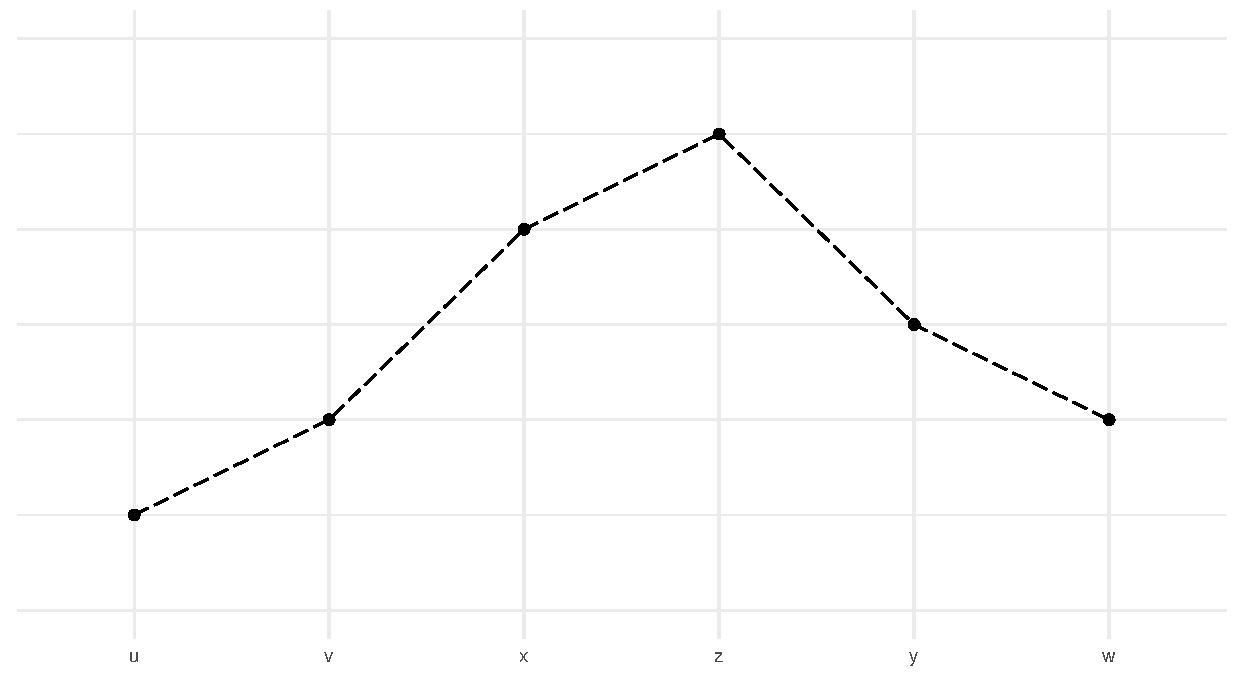
\includegraphics[scale=0.5]{images/Ex3.5(a)1.pdf}
\end{center}

Consider preference $zPxPyPwIvPu$, is it single-peaked with respect to $v>w>y>z>x>u$?

\begin{center}
    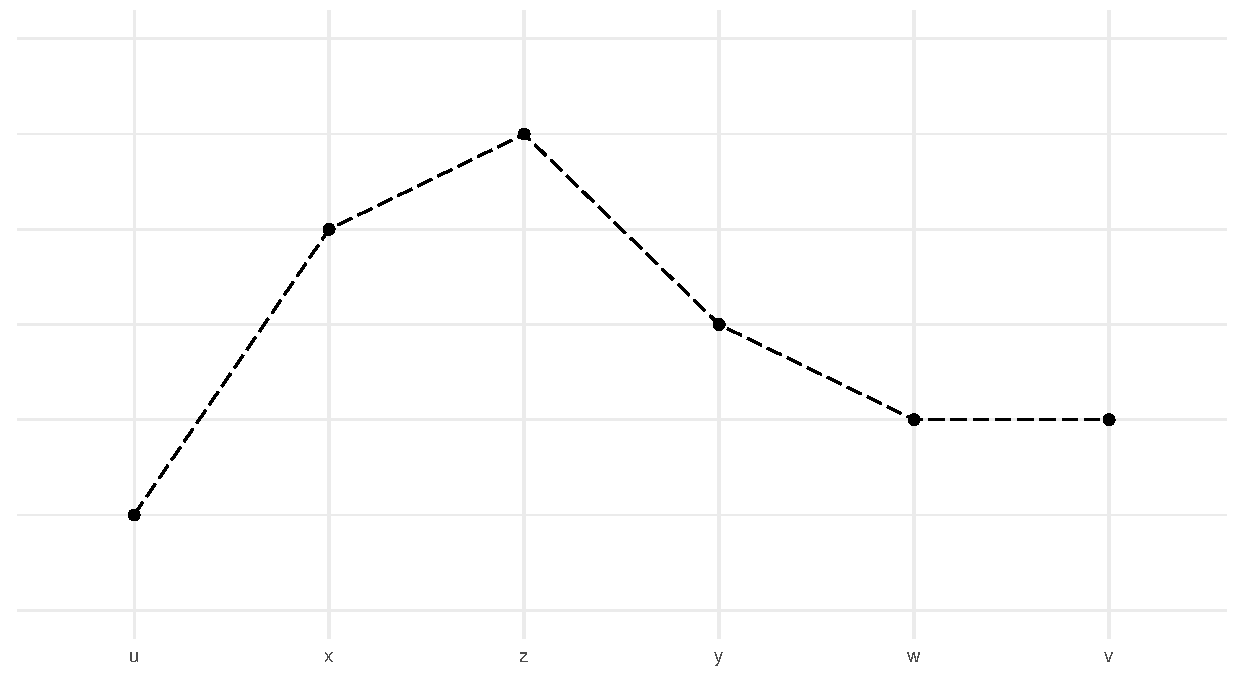
\includegraphics[scale=0.5]{images/Ex3.5(a)2.pdf}
\end{center}

In order to make the preference single-peaked, any indifference between two alternatives must arise across different sides of the peak. Hence, the preference $zPxPyPwIvPu$ is NOT single-peaked with respect to $v>w>y>z>x>u$.

\subsubsection*{(b)}

Consider preference $yPwIzPvIx$, is it single-peaked with respect to some order?
\begin{center}
    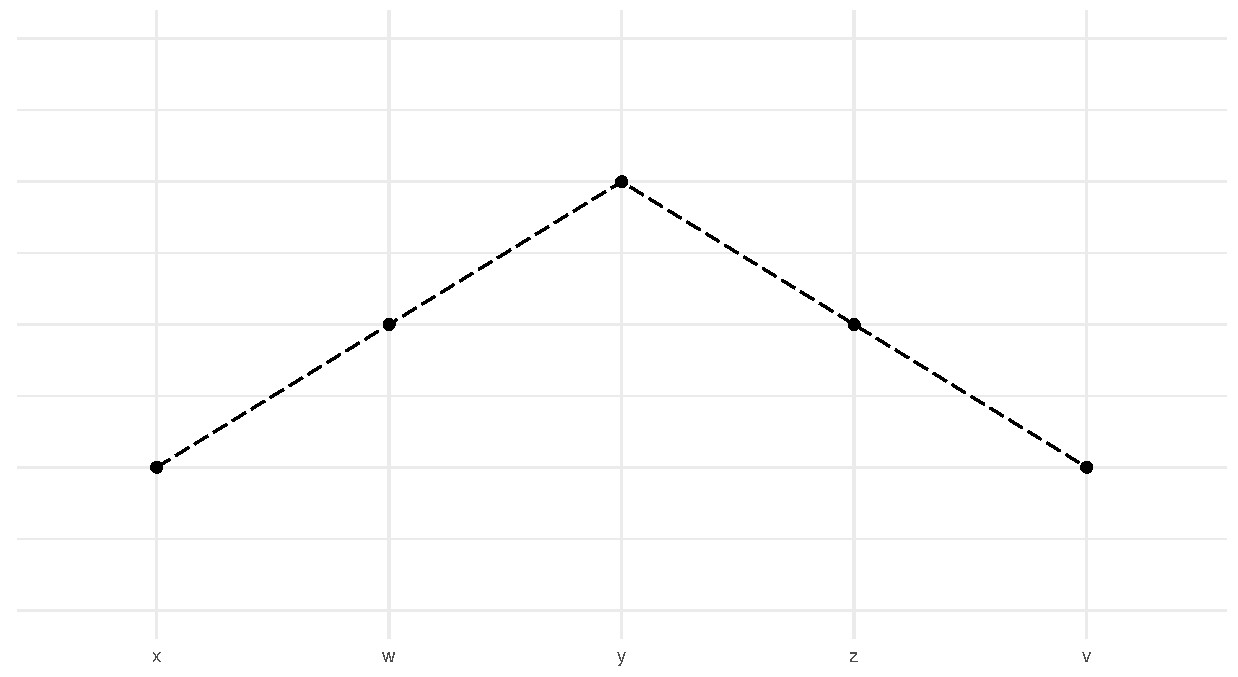
\includegraphics[scale=0.5]{images/Ex3.5(b)1.pdf}
\end{center}

There are four different orders that make preference $yPwIzPvIx$ single-peaked:
\begin{itemize}
    \item $v>z>y>w>x$
    \item $x>w>y>z>v$
    \item $v>w>y>z>x$
    \item $x>z>y>w>v$
\end{itemize}


Consider preference $yPwIzIvPx$, is it single-peaked with respect to some order?
\begin{center}
    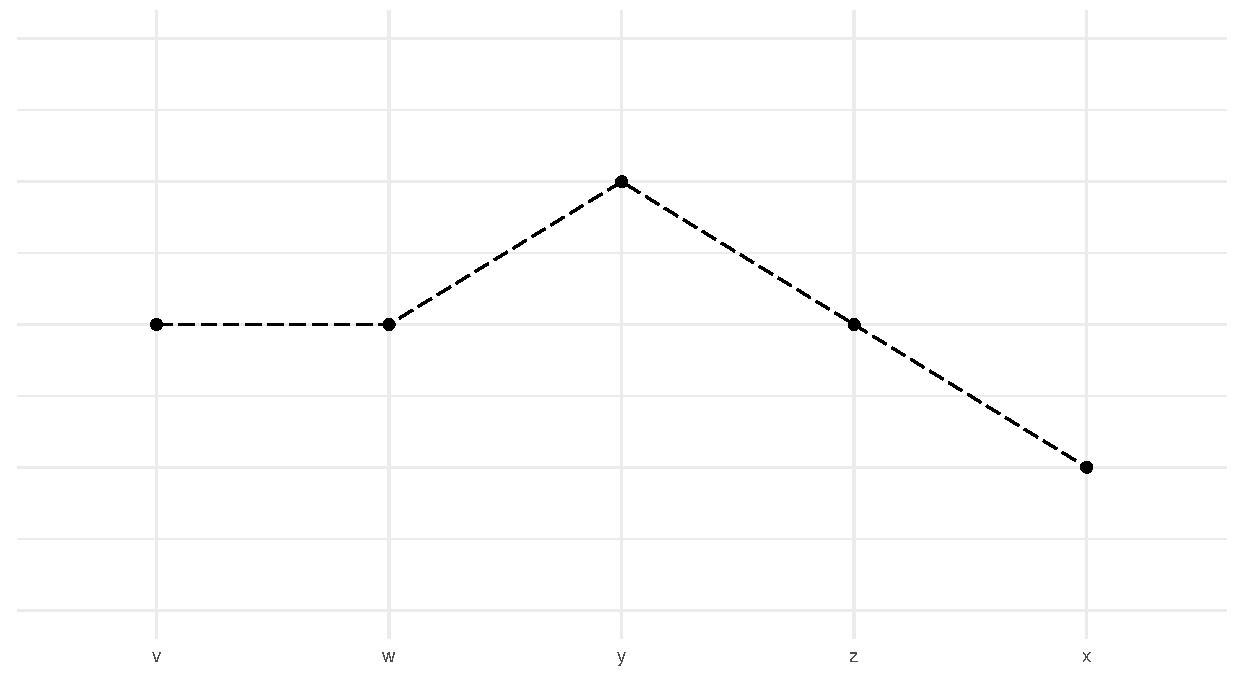
\includegraphics[scale=0.5]{images/Ex3.5(b)2.pdf}
\end{center}

There are three indifferent alternatives. No matter how we allocate these indifferent alternatives across the peak, we are not able to construct the single-peaked preference with respect to any order.

\subsection*{Exercise 3.6}

\subsubsection*{(a)}

\begin{table}[!htbp]
    \centering
    \begin{tabular}{c|c|}
        \# & preferences         \\ 
        \hline
        1  & $x\: P\: y\: P\: z$ \\
        1  & $y\: P\: z\: P\: x$ \\
        1  & $y\: P\: x\: P\: z$ \\
        \hline
    \end{tabular}
\end{table}

Are these preferences single-peaked with respect to $y>x>z$?
\begin{center}
    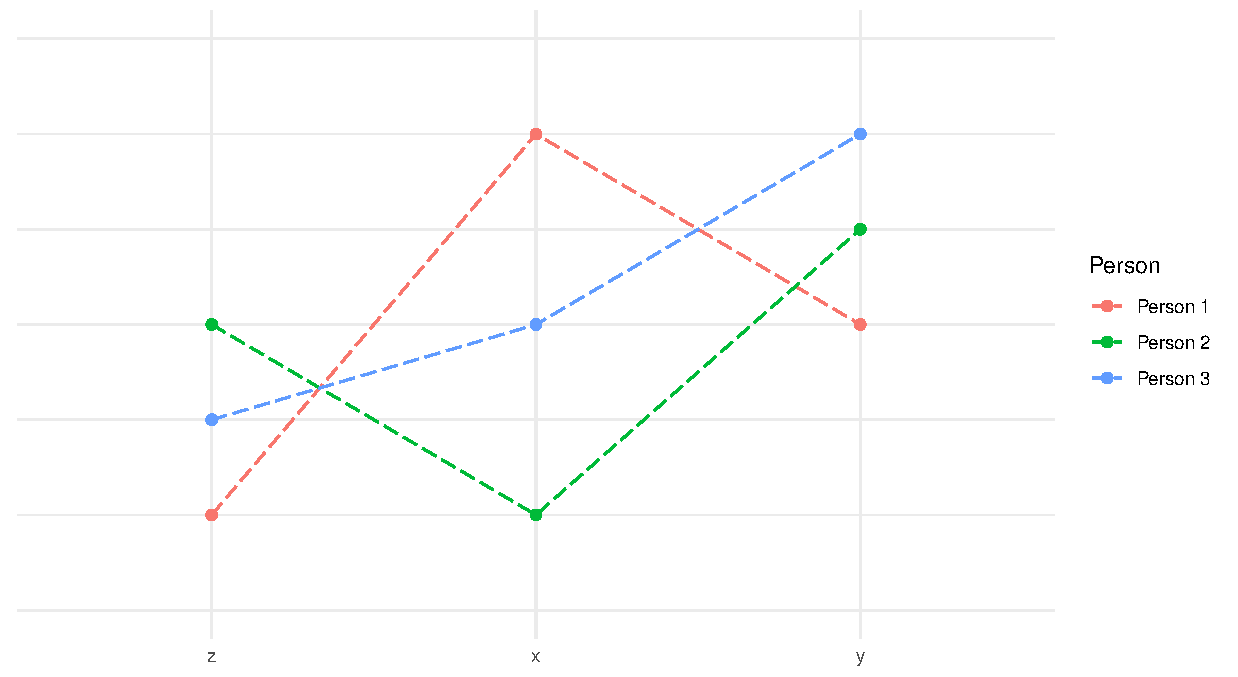
\includegraphics[scale=0.5]{images/Ex3.6(a)1.pdf}
\end{center}

As we can see from the graph, Person 2's preference is not single-peaked (there is a dip in the middle).

Is there an order with respect to which they are all single-peaked?
\begin{center}
    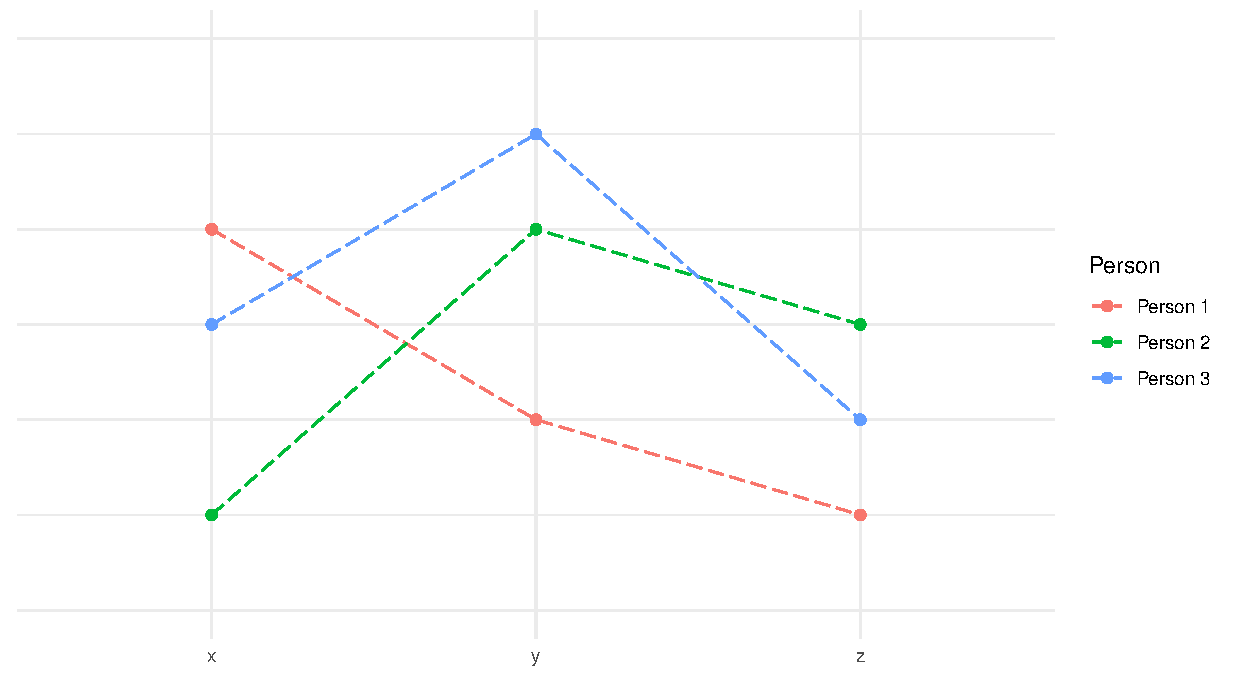
\includegraphics[scale=0.5]{images/Ex3.6(a)2.pdf}
\end{center}

Idea: $x$ and $z$ are bottom-ranked by at least one person, so we cannot put these two alternatives in the middle, otherwise we would immediately get a violation of single-peaked preferences. 
\begin{itemize}
    \item $z>y>x$
    \item $x>y>z$
\end{itemize}

\subsubsection*{(b)}

\begin{table}[!htbp]
    \centering
    \begin{tabular}{c|c|}
        \# & preferences         \\ 
        \hline
        1  & $x\: P\: y\: P\: z$ \\
        1  & $y\: P\: z\: P\: x$ \\
        1  & $z\: P\: x\: P\: y$ \\
        \hline
    \end{tabular}
\end{table}

Is there an order with respect to which these preferences are single-peaked?

\begin{itemize}
    \item Each alternative is bottom-ranked at least by one individual. No matter which order we use, there always exist at least one individual whose preference is not single-peaked.
    \item We can easily see that preferences are cyclical. By the Median Voter Theorem, the median voter (i.e., Condorcet winner) does not exist and the number of voters is odd, hence preferences cannot be single-peaked.
\end{itemize}

\subsection*{Exercise 3.7}

\begin{table}[!htbp]
    \centering
    \begin{tabular}{c|c|}
        \# & preferences         \\ 
        \hline
        2  & $w\: P\: x\: P\: y\: P\: z$ \\
        2  & $x\: P\: y\: P\: z\: P\: w$ \\
        1  & $y\: P\: z\: P\: x\: P\: w$ \\
        \hline
    \end{tabular}
\end{table}

\subsubsection*{(a)}

$z$ and $w$ are bottom-ranked by at least one individual so we cannot order them in the middle. Since there are only four alternatives, we can only put $z$ and $w$ on the two sides of the order. Note that the first two people have exactly the preferences as described before. Hence, we must respect the order of preferences for the first two people, otherwise we would get immediate violation of single-peaked preferences.

\begin{center}
    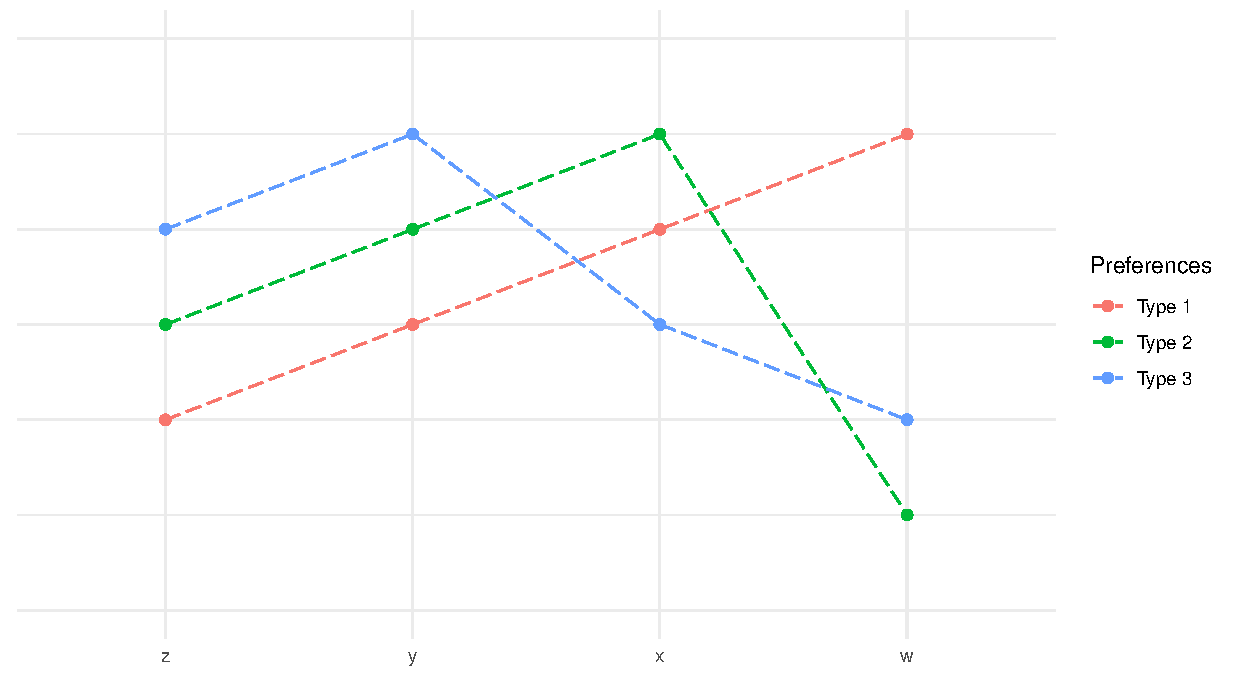
\includegraphics[scale=0.5]{images/Ex3.7(a).pdf}
\end{center}

\begin{itemize}
    \item $w>x>y>z$
    \item $z>y>x>w$
\end{itemize}

\subsubsection*{(b)}

Apply pairwise majority voting. Is there a Condorcet winner/loser?

\begin{table}[!htbp]
    \centering
    \begin{tabular}{ccc}
    pairwise comparison & votes & social preference $f^\text{PM}$  \\
    \hline 
    $x:w$               & $3:2$ & $xPw$                            \\
    $y:w$               & $3:2$ & $yPw$                            \\
    $z:w$               & $3:2$ & $zPw$                            \\
    $x:y$               & $4:1$ & $xPy$                            \\
    $x:z$               & $4:1$ & $xPz$                            \\
    $y:z$               & $5:0$ & $yPz$                            \\
    \hline
    \end{tabular}
\end{table}

Social welfare function: $xPyPzPw$
\begin{itemize}
    \item $x$ is the Condorcet winner
    \item $w$ is the Condorcet loser
\end{itemize}

\subsubsection*{(c)}
\begin{itemize}
    \item $x$ is the median voters' peak
    \item Median voters are those who choose $x$ as their top rank
\end{itemize}

\section*{Part 4: Individual Rights}

\subsection*{Exercise 4.1}

\begin{table}[!htbp]
    \centering
    \begin{tabular}{c|c|c|}
    \backslashbox{1}{2} & $C$  & $O$  \\
    \hline
    $C$                 & $CC$ & $CO$ \\
    \hline
    $O$                 & $OC$ & $OO$ \\
    \hline
    \end{tabular}
\end{table}

\subsubsection*{(a)}

The rights system $\mathbf{D}=(D_1,D_2)$
\begin{align*}
    D_1 &= \{(CC, OC), (OC, CC), (CO, OO), (OO, CO) \} \\
    D_2 &= \{(CC, CO), (CO, CC), (OC, OO), (OO, OC) \}
\end{align*}

\subsubsection*{(b)}

A preference profile $\mathbf{R}=(R_1, R_2)$
\begin{align*}
    & R_1: CO \succ OO \succ CC \succ OC \\
    & R_2: OC \succ OO \succ CC \succ CO
\end{align*}

\begin{itemize}
    \item $CC \succ OC$ because of $D_1$
    \item $OC \succ OO$ because of $D_2$
    \item $OO \succ CC$ because of $[\text{P}^*]$
\end{itemize}

This preference profile $\mathbf{R}$ leads to an outcome that is cyclical (Prisoner's dilemma)

\section*{Part 5: Manipulability}

\subsection*{Exercise 5.1}

\begin{table}[!htbp]
    \centering
    \begin{tabular}{c|c|cccc|}
        \# & true preferences             & $w$  & $x$  & $y$  & $z$ \\ 
        \hline
        1  & $x\: P\: y\: P\: z\: P\: w$  & $0$  & $3$  & $2$  & $1$ \\
        1  & $y\: P\: z\: P\: w\: P\: x$  & $1$  & $0$  & $3$  & $2$ \\
        1  & $y\: P\: w\: P\: z\: P\: x$  & $2$  & $0$  & $3$  & $1$ \\
        \hline
           &                              & $3$ & $3$  & $8$  & $4$ \\
        \hline
    \end{tabular}
\end{table}

\begin{itemize}
    \item Person 2 and Person 3 do not benefit from voting non-truthfully
    \item Person 1 cannot make $x$ win even if he manipulates by dropping $y$ as her bottom rank
\end{itemize}

\begin{table}[!htbp]
    \centering
    \begin{tabular}{c|c|cccc|}
        \# & true preferences             & $w$  & $x$  & $y$  & $z$ \\ 
        \hline
        1  & $y\: P\: z\: P\: x\: P\: w$  & $0$  & $1$  & $3$  & $2$ \\
        1  & $z\: P\: y\: P\: x\: P\: w$  & $0$  & $1$  & $2$  & $3$ \\
        1  & $w\: P\: z\: P\: y\: P\: x$  & $3$  & $0$  & $1$  & $2$ \\
        \hline
           &                              & $3$ & $2$  & $6$  & $7$ \\
        \hline
    \end{tabular}
\end{table}

Manipulation:
\begin{table}[!htbp]
    \centering
    \begin{tabular}{c|c|cccc|}
        \# & ballot                       & $w$  & $x$  & $y$  & $z$ \\ 
        \hline
        1  & $y\: P\: x\: P\: w\: P\: z$  & $1$  & $2$  & $3$  & $0$ \\
        1  & $z\: P\: y\: P\: x\: P\: w$  & $0$  & $1$  & $2$  & $3$ \\
        1  & $w\: P\: z\: P\: y\: P\: x$  & $3$  & $0$  & $1$  & $2$ \\
        \hline
           &                              & $4$ & $3$  & $6$  & $5$ \\
        \hline
    \end{tabular}
\end{table}

\begin{itemize}
    \item Person 1 can successfully manipulate by ranking $x$ at the last position while maintaining other alternatives their relative position.
    \item Person 2 cannot benefit from manipulation and does have any incentive to do so as she gets his top-ranked alternative in truthful voting.
    \item Person 3 cannot make $w$ win as $w$ is already top-ranked by her.
\end{itemize}

As a side note:

Person 2 can strengthen her top-ranked alternative by deliberately ranking $y$ as bottom to avoid any potential manipulation from others

\begin{table}[!htbp]
    \centering
    \begin{tabular}{c|c|cccc|}
        \# & ballot                       & $w$  & $x$  & $y$  & $z$ \\ 
        \hline
        1  & $y\: P\: z\: P\: x\: P\: w$  & $0$  & $1$  & $3$  & $2$ \\
        1  & $z\: P\: x\: P\: w\: P\: y$  & $1$  & $2$  & $0$  & $3$ \\
        1  & $w\: P\: z\: P\: y\: P\: x$  & $3$  & $0$  & $1$  & $2$ \\
        \hline
           &                              & $4$ & $3$  & $4$  & $7$ \\
        \hline
    \end{tabular}
\end{table}

\subsection*{Exercise 5.2}

\textit{Assume $n=2$ and $m=3$. The following table completely specifies an SCF on the domain of strict preferences ($\mathscr{A}=\mathscr{P}^n$)}
\begin{table}[!htbp]
    \centering
    \begin{tabular}{c|c|c|c|c|c|c|}
    \backslashbox{$R_1$}{$R_2$} & $xyz$ & $xzy$ & $yxz$ & $yzx$ & $zxy$ & $zyx$ \\
    \hline
    $xyz$                       & $x$   & $x$   & $x$   & $x$   & $x$   & $x$   \\
    \hline
    $xzy$                       & $x$   & $x$   & $x$   & $x$   & $x$   & $x$   \\
    \hline
    $yxz$                       & $x$   & $x$   & $y$   & $y$   & $x$   & $y$   \\
    \hline
    $yzx$                       & $x$   & $x$   & $y$   & $y$   & $y$   & $y$   \\
    \hline
    $zxy$                       & $x$   & $x$   & $x$   & $y$   & $z$   & $z$   \\
    \hline
    $zyx$                       & $x$   & $x$   & $y$   & $y$   & $z$   & $z$   \\
    \hline
    \end{tabular}
\end{table}

\subsection*{Exercise 5.3}

\begin{table}[!htbp]
    \centering
    \begin{tabular}{c|c|}
        \# & true preferences         \\ 
        \hline
        1  & $y\: P\: x\: P\: z$ \\
        1  & $z\: P\: x\: P\: y$ \\
        \hline
    \end{tabular}
\end{table}

\begin{table}[!htbp]
    \centering
    \begin{tabular}{c|c|}
        \# & ballot              \\ 
        \hline
        1  & $y\: P\: x\: P\: z$ \\
        1  & $x\: P\: y\: P\: z$ \\
        \hline
    \end{tabular}
\end{table}

\begin{itemize}
    \item If everyone votes truthfully, we will get equal votes for $y$ and $z$. According to the tie-breaking rule, $y$ would be preferred by society. 
    \item However, Person 2 has an incentive to manipulate by ranking $z$ as bottom. If so, there will be a tie between $x$ and $y$. According to the tie-breaking rule, the society would prefer $x$ in this case. For Person 2, $x$ is better than $y$, hence a successful manipulation.
\end{itemize}

\section*{Part 6: Distributive Justice}

\subsection*{Exercise 6.1}

Overview of Information Structures:
\begin{table}[!htbp]
    \centering
    \begin{tabular}{l|c|c|c|}
                               & no comparability & unit comparability & level comparability \\ 
        \hline
        ordinal measurability  & OM-NC            &                    & OM-LC               \\
        \hline
        cardinal measurability & CM-NC            & CM-UC              & CM-LC               \\
        \hline
        ratio measurability    & RM-NC            &                    & RM-LC               \\
        \hline
    \end{tabular}
\end{table}

\subsubsection*{(a)}

Pareto inefficient set:
\[X^{I}(\mathbf{U})=\left\{x\in X \mid \exists y\in X \text{ s.t. } U_i(y)\geq U_i(x) \text{ and } U_j(y)>U_j(x) \text{ for some } j \right\} \]

Pareto efficient set:
\[X^{E}(\mathbf{U})=X\setminus X^{I}(\mathbf{U}) \]

OM-NC:

Suppose $U_i'=\phi_i(U_i)$ where $\phi_i$ is a strictly increasing transformation function, then
\begin{align*}
    X^I(\mathbf{U}') &= X^I(\mathbf{U}) \\
    X^E(\mathbf{U}') &= X^E(\mathbf{U})
\end{align*}
Note that Pareto efficiency comparison does not involve any utility comparison across people.

\subsubsection*{(b)}

The Nash SEF $e^{NA}$ that selects the preference represented by
\[NA(x,\mathbf{U})=\prod_{i=1}^{n} U_i(x), \qquad \forall x\in X, \mathbf{U}\in\mathscr{U}^{n} \]

RM-NC:

Suppose $U_i'=\beta_iU_i$ where $\beta_i>0$,
\begin{align*}
    NA(x,\mathbf{U}') &= \prod_{i=1}^{n}U_i'(x) \\
    &= \prod_{i=1}^{n}\beta_i U_i(x) \\
    &= \underbrace{\prod_{i=1}^{n}\beta_i}_{\beta>0} \cdot \underbrace{\prod_{i=1}^{n}U_i(x)}_{NA(x,\mathbf{U})} \\
    &= \beta \cdot NA(x,\mathbf{U})
\end{align*}

CM-LC:

Common positive affine transformation: $\alpha=3, \beta=1$
\[U_i'=\alpha + \beta U_i \]
\begin{table}[!htbp]
    \centering
    \begin{tabular}{c|cc|}
        $\mathbf{U}$ & $x$ & $y$              \\ 
        \hline
        $U_1$        & $1$ & $2$ \\
        $U_2$        & $5$ & $3$ \\
        \hline
        $NA(x,\mathbf{U})$ & $5$ & $6$ \\
    \end{tabular}
    $\qquad\qquad$
    \begin{tabular}{c|cc|}
        $\mathbf{U'}$ & $x$ & $y$              \\ 
        \hline
        $U_1'$        & $4$ & $5$ \\
        $U_2'$        & $8$ & $6$ \\
        \hline
        $NA(x,\mathbf{U}')$ & $32$ & $30$ \\
    \end{tabular}
\end{table}

\subsubsection*{(c)}

The isoelastic SEF $e^{IE}$ that selects the preference represented by
\[IE(x,\mathbf{U})=\frac{1}{1-\rho}\sum\left(U_i(x) \right)^{1-\rho},\qquad\forall x\in X,\mathbf{X}\in\mathscr{U}^{n} \]

\begin{equation*}
    \frac{1}{1-\rho}\sum\left(U_i(x) \right)^{1-\rho}=
    \begin{cases}
        \sum_{i=1}^{n}U_i(x), & \rho=0 \\
        \log \left(\prod_{i=1}^{n} U_i(x) \right), & \rho=1 \\
        \min\left\{U_1(x),\cdots, U_n(x) \right\}, & \rho=\infty
    \end{cases}
\end{equation*}

\begin{equation*}
    IE(x,\mathbf{U})=
    \begin{cases}
        UT(x,\mathbf{U}), & \rho=0 \\
        \log \left(NA(x,\mathbf{U})\right), & \rho=1 \\
        MM(x,\mathbf{U}), & \rho=\infty
    \end{cases}
\end{equation*}

RM-LC:

$U_i'(x)=\beta U_i(x)\quad\forall i$
\begin{align*}
    IE(x, \mathbf{U}') &= \frac{1}{1-\rho}\sum_{i=1}^{n}(U_i'(x))^{1-\rho} \\
    &= \frac{1}{1-\rho}\sum_{i=1}^{n}(\beta U_i(x))^{1-\rho}      \\
    &= \frac{1}{1-\rho}\sum_{i=1}^{n}\beta^{1-\rho}\cdot (U_i(x))^{1-\rho} \\
    &= \frac{\beta^{1-\rho}}{1-\rho}\sum_{i=1}^{n}(U_i(x))^{1-\rho} \\
    &= \underbrace{\beta^{1-\rho}}_{>0}\cdot IE(x,\mathbf{U})
\end{align*}

\newpage

RM-NC:

Assume $\rho=\frac{1}{2}$
\[IE(x,\mathbf{U})=2\sum\sqrt{U_i(x)},\qquad\forall x\in X,\mathbf{X}\in\mathscr{U}^{n} \]

Individual-specific positive linear transformation: $\beta_1=4,\beta_2=25$
\begin{table}[!htbp]
    \centering
    \begin{tabular}{c|cc|}
        $\mathbf{U}$ & $x$ & $y$              \\ 
        \hline
        $U_1$        & $4$ & $36$ \\
        $U_2$        & $25$ & $9$ \\
        \hline
        $IE(x,\mathbf{U})$ & $14$ & $18$ \\
    \end{tabular}
    $\qquad\qquad$
    \begin{tabular}{c|cc|}
        $\mathbf{U'}$ & $x$ & $y$              \\ 
        \hline
        $U_1'$        & $4^2$ & $12^2$ \\
        $U_2'$        & $25^2$ & $15^2$ \\
        \hline
        $IE(x,\mathbf{U}')$ & $58$ & $54$ \\
    \end{tabular}
\end{table}

CM-LC:

common positive affine transformation: $\alpha=1, \beta=1$
\begin{table}[!htbp]
    \centering
    \begin{tabular}{c|cc|}
        $\mathbf{U}$ & $x$ & $y$              \\ 
        \hline
        $U_1$        & $4$ & $16$ \\
        $U_2$        & $100$ & $64$ \\
        \hline
        $IE(x,\mathbf{U})$ & $24$ & $24$ \\
    \end{tabular}
    $\qquad\qquad$
    \begin{tabular}{c|cc|}
        $\mathbf{U'}$ & $x$ & $y$              \\ 
        \hline
        $U_1'$        & $5$ & $17$ \\
        $U_2'$        & $101$ & $65$ \\
        \hline
        $IE(x,\mathbf{U}')$ & $24.57$ & $24.37$ \\
    \end{tabular}
\end{table}

\begin{table}[!htbp]
    \centering
    \begin{tabular}{l|c|c|c|}
                               & no comparability & unit comparability & level comparability \\ 
        \hline
        ordinal measurability  & BC, EM           &                    & Maximin             \\
        \hline
        cardinal measurability &                  & Utilitarian        &                     \\
        \hline
        ratio measurability    & Nash SEF         &                    & Isoelastic SEF      \\
        \hline
    \end{tabular}
\end{table}

\end{document}
